\documentclass[UTF-8]{ctexart}

\usepackage{amsmath}
\newtheorem{definition}{Definition}[section]
\newtheorem{theorem}{Theorem}[section]
\newtheorem{lemma}{Lemma}
\newtheorem{proof}{Proof}[section]

\usepackage{graphicx} %插入图片的宏包
\usepackage{float} %设置图片浮动位置的宏包
\usepackage{subfigure} %插入多图时用子图显示的宏包

% 开始文档
\begin{document}

% 创建标题页的内容
\title {数学学习笔记} \author{cpd} \date{2023/11/12}
% 生成标题
\maketitle

% 设置页码格式是罗马数字
\pagenumbering{roman}
% 生成目录
\tableofcontents
% 插入新页
\newpage
% 设置页码格式是阿拉伯数字
\pagenumbering{arabic}

% 下面是章节
\section{定义}

% 分节
% \subsection{点积}
\begin{definition}
  the dot product or inner product of $\mathbf{v}
=(v_1,v_2)$and$\mathbf{w}=(w_1,w_2)$is the number $\mathbf{v} \cdot \mathbf{w} = v_1w_1+v_2w_2$.

\end{definition}
\section{定理}

\begin{theorem}
  点积为零表示两个向量垂直.

\end{theorem}
\begin{proof}
  \begin{figure}[H] %H为当前位置,!htb为忽略美学标准,htbp为浮动图形
    \centering %图片居中
    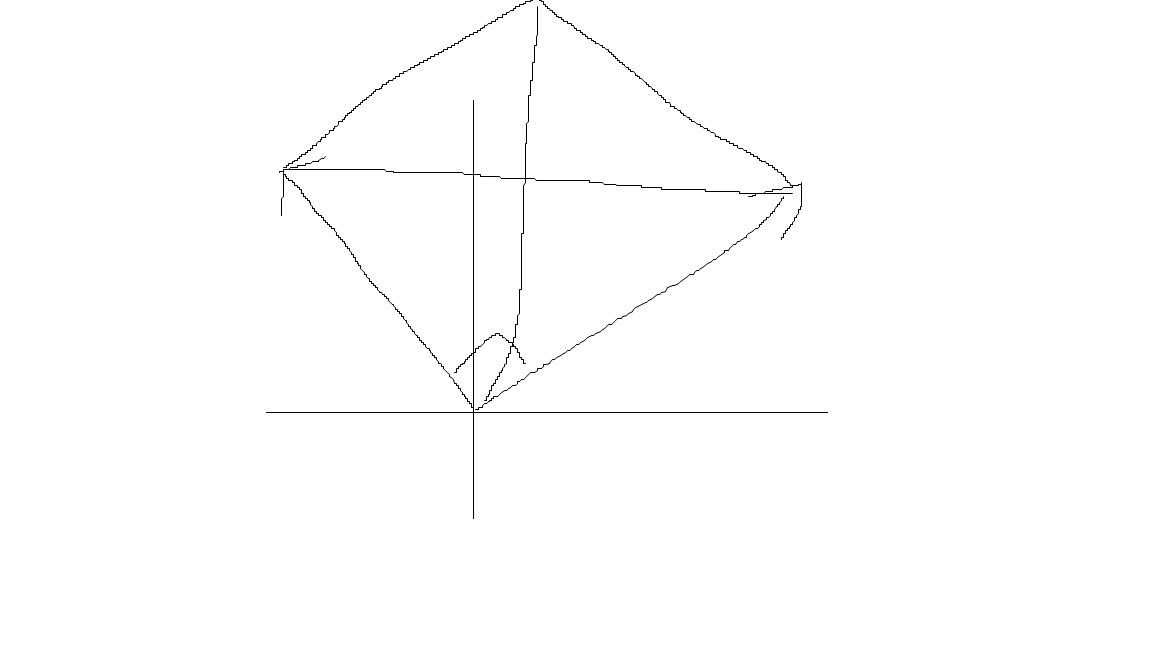
\includegraphics[width=0.7\textwidth]{images/math/1.jpg} %插入图片,[]中设置图片大小,{}中是图片文件名
    % \caption{Main name 2} %最终文档中希望显示的图片标题
    % \label{Fig.main2} %用于文内引用的标签
  \end{figure}
  由于两个向量组成了直角三角形,由勾股定理可知斜边长的平方
  为$v_1^2+v_2^2+w_1^2+w_2^2$. 由于矩形的两个对角线相等,所以该斜边长等于另一个对角
  线的长度. 另一个对角线的终点坐标
  为$(v_1+w_1,v_2+w_2)$,所以$v_1^2+v_2^2+w_1^2+w_2^2=(v_1+w_1)^2+(v_2+w_2)^2$,化简
  即可得$v_1w_1+v_2w_2=0$. $v_1$	
\end{proof}


\end{document}
